%!TEX root=../report.tex

\section{Experiments and Evaluation}

Dynamic simulations are a method to support a hypothesis. In the context of Uno I will analyze the questions How many rounds does it take to finish the game?
This kind of question are useful for game developers when they have to balance the game. For instance a game like uno should take to long, because it is designed for kids.
The second part is dedicated to the verification and validation of the model. Regarding validation I analyze the role of player behavior and compare simplified Uno with the offical Uno implementation.

\subsection{Analyzing the variables of the game}

\note{pattern of draw pile etc.}


\subsection{How many rounds does it take to finish Uno?}

At first I want to find out how the number of cards that you get initially impacts the duration of the game. 

\begin{figure}[h!]
  \caption{\note{number of turns to finish the game}}
  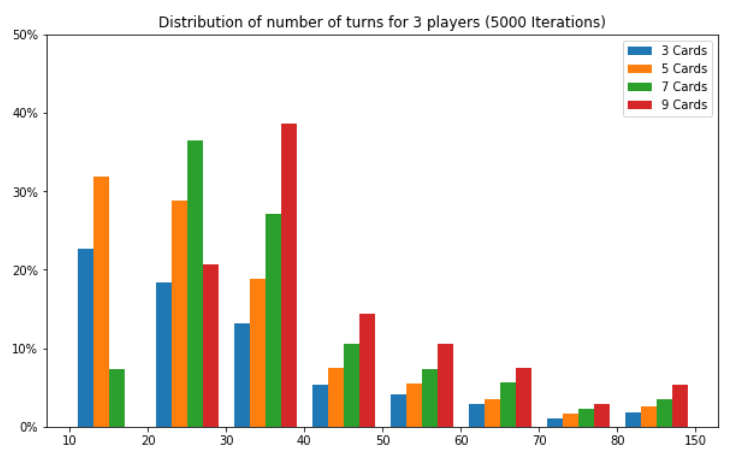
\includegraphics[width=0.9\textwidth]{histogram-cards}
\end{figure}


The histogram shows bars and percentage of games that end after 10-20 turns, 20-30 and so on. The more cards, the longer takes the game. The probability to finish after less than 20 turns is a bit to high with 3 or 5 cards in the beginning. 7 cards would mean that more than 50\% of the games would end after 20-40 turns.


Second analysis the impact of the number of players. I simulate Uno with 7 cards per player and 2-6 players per game. The histograms show the percentage of games that end with 10 to 20 turns, or 20 to 30 turns and so on. The last interval is from 80 to 150. You can see that most games end after 30-40 turns. And more player automatically leads to more turns, thats why I normalized the distribution by the number of players. Et voila, with 6 players it is very likely that the game ends in less than 20 rounds while with two players games can be very long. So 7 cards seems also be ok from this perspective, but maybe it’s worth to think about a 2-player version and name it Uno - Das Duell.


\begin{figure}[h!]
  \caption{\note{number of turns to finish the game}}
  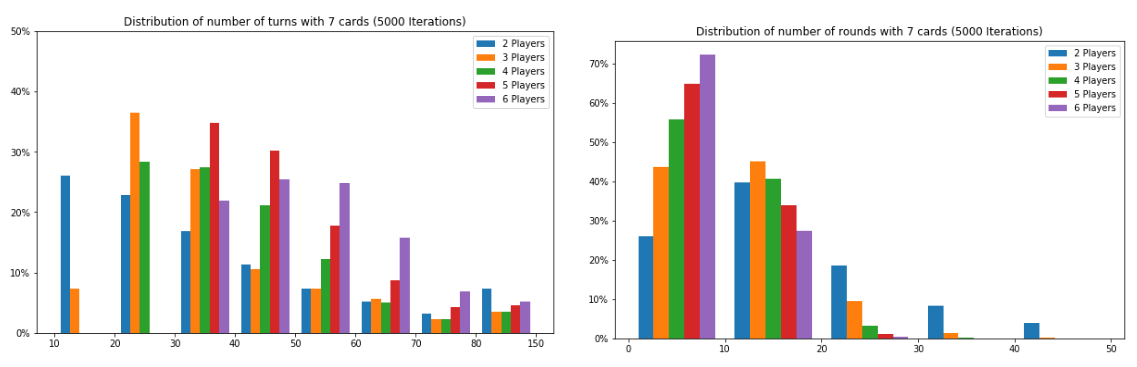
\includegraphics[width=0.9\textwidth]{histogram-players}
\end{figure}

\subsection{Verification and Validation}


One interesting question here is how often should I run the simulation. I observed the standard deviation every 100 iterations and it divergates after 5000

Last step is to analyze the result. 

Regargding Validation we can check for the three R’s.
(1) reality — how the model closely matches reality. The players in the game are simulated with a very simple and equal behavior. This won’t be the case in the real world. But the overall structure of the game exists.
(2) representation — some aspects are represented, some are not. I covered the basic concept but I decided to incorperate all special rules. This would increase the complexity but may not change the actual flow of the game.
(3) requirements — different levels of fi delity required for different applications. The requirement of the model was to answer the question of how many rounds does a game take and how could this be used for game balancing. This is also the reason why some aspects are not represented. E.g. thinking time or forget to say uno.

